\chapter{Uncertainty and Error Part 1}
\label{chap:excel}
\section{Introduction}

There is no such thing as a perfect measurement. All measurements have errors and uncertainties, no matter how hard we might try to minimize them. Understanding possible errors is an important issue in any experimental science. The conclusions we draw from the data, and especially the strength of those conclusions, will depend on how well we control the uncertainties. \myskip

Let’s look at an \emph{example}: You measure two values 2.5 and 1.5. From theory, the expected value is 2.3, so the value 2.5 almost agrees, whereas 1.5 is far off. But if you take into account the uncertainties (i.e.\ the interval in which your result is expected to lie), neither may be far off. For experimental uncertainties of 0.1 and 1.0, respectively, your two measured values may be expressed $2.5\pm 0.1$ and $1.5\pm 1.0$. The expected value falls within the range of the second measurement but not of the first! \myskip

Analyzing data and error in experiments is essential in making conclusions about the physical laws we are testing. The advent of computers and software made to manipulate large data sets has revolutionized scientist's ability to make conclusions from experimental data. In this lab course, we will be using Microsoft Excel to record data sets from the experiments and determine experimental uncertainties in calculated quantities. We will learn to use excel to propagate uncertainties and plot error bars with our data. You can download a personal copy of Microsoft Excel with your student email address from 
\href{https://products.office.com/en-us/student?ms.officeurl=getoffice365}{Office 365 Education} \footnote{https://products.office.com/en-us/student?ms.officeurl=getoffice365}. Please note the sections introducing new Excel tools pertain to the newest version of Excel. If you are using a personal computer with a different version of Excel, you are responsible for adapting the instructions to your version of Excel. \myskip

The purpose of this first lab is to introduce some basic information about statistics and error in experiments and to show how we can use excel to represent error in data. The techniques studied here will be essential for the rest of this two-semester lab course. The issues and techniques are important in order to arrive at good judgments in any field (like medicine) in which it is necessary to understand not just numerical results, but the uncertainties associated with those results.

\section{Theory- Uncertainty and Error}

\subsection{Types of Uncertainties}

Uncertainty in a measurement can arise from three possible origins: the measuring device, the procedure of how you measure, and the observed quantity itself. Usually the largest of these will determine the uncertainty in your data. \myskip

Uncertainties can be divided into two different types: systematic uncertainties and random uncertainties. 

\subsubsection{Systematic Uncertainties}

Systematic uncertainties or systematic errors always bias results in one specific direction. They will cause your measurement to consistently be higher or lower than the accepted value. \myskip

An \emph{example} of a systematic error follows. Assume you want to measure the length of a table in cm using a meter stick. However, the stick is made of metal that has contracted due to the temperature in the room, so that it is less than one meter long. Therefore, all the intervals on the stick are smaller than they should be. Your numerical value for the length of the table will then always be larger than its actual length no matter how often or how carefully you measure. Another example might be measuring temperature using a mercury thermometer in which a bubble is present in the mercury column. \myskip

Systematic errors are usually due to imperfections in the equipment, improper or biased observation, or the presence of additional physical effects not taken into account. (An example might be an experiment on forces and acceleration in which there is friction in the setup and it is not taken into account!) \myskip

In performing experiments, try to estimate the effects of as many systematic errors as you can, and then remove or correct for the most important. By being aware of the sources of systematic error beforehand, it is often possible to perform experiments with sufficient care to compensate for weaknesses in the equipment.

\subsubsection{Random Uncertainties}

In contrast to systematic uncertainties, random uncertainties are an unavoidable result of measurement, no matter how well designed and calibrated the tools you are using. Whenever more than one measurement is taken, the values obtained will not be equal but will exhibit a spread around a mean value, which is considered the most reliable measurement. That spread is known as the random uncertainty. Random uncertainties are also unbiased -- meaning it is equally likely that an individual measurement is too high or too low. \myskip

From your everyday experience you might be thinking, ``Stop! Whenever I measure the length of a table with a meter stick I get exactly the same value no matter how often I measure it!''   This may happen if your meter stick is insensitive to random measurements, because you use a coarse scale (like $\mathrm{mm}$) and you always read the length to the nearest $\mathrm{mm}$. But if you would use a meter stick with a finer scale, or if you interpolate to fractions of a millimeter, you would definitely see the spread. As a general rule, if you do not get a spread in values, you can improve your measurements by using a finer scale or by interpolating between the finest scale marks on the ruler. \myskip

How can one reduce the effect of random uncertainties?  Consider the following \emph{example}. Ten people measure the time of a sprinter using stopwatches. It is very unlikely that each of the ten stopwatches will show exactly the same result. Even if all of the people started their watches at exactly the same time (unlikely) some of the people will have stopped the watch early, and others may have done so late. You will observe a spread in the results. If you \emph{average} the times obtained by all ten stop watches, the \emph{mean} value will be a better estimate of the true value than any individual measurement, since the uncertainty we are describing is random, the effects of the people who stop early will compensate for those who stop late. In general, making multiple measurements and averaging can reduce the effect of random uncertainty. \myskip

\emph{Remark}: We usually specify any measurement by including an estimate of the random uncertainty. (Since the random uncertainty is unbiased we note it with a $\pm$ sign). So if we measure a time of 7.6 seconds, but we expect a spread of about 0.2 seconds, we write as a result:
\begin{equation}
    t = (7.6\pm 0.2)\,\mathrm{s}
\end{equation}
indicating that the uncertainty of this measurement is $0.2\,\mathrm{s}$ or about $3\%$. \myskip
\subsection{Accuracy and Precision}
An important distinction in physics is the difference between the {\it{accuracy}} and the {\it{precision }} of a measurement.
Accuracy refers to the closeness of a measured value to a standard or known value. For example, if in lab you obtain a weight measurement of 3.2 kg for a given substance, but the actual or known weight is 10 kg, then your measurement is not accurate. In this case, your measurement is not close to the known value. \myskip

Precision refers to the closeness of two or more measurements to each other. Using the example above, if you weigh a given substance five times, and get 3.2 kg each time, then your measurement is very precise. Precision is independent of accuracy. You can be very precise but inaccurate, as described above. You can also be accurate but imprecise. \myskip

For example, if on average, your measurements for a given substance are close to the known value, but the measurements are far from each other, then you have accuracy without precision. \myskip

A good analogy for understanding accuracy and precision is to imagine a basketball player shooting baskets. If the player shoots with accuracy, his aim will always take the ball close to or into the basket. If the player shoots with precision, his aim will always take the ball to the same location which may or may not be close to the basket. A good player will be both accurate and precise by shooting the ball the same way each time and each time making it in the basket. 
\subsection{Numerical Estimates of Uncertainties}

For this laboratory, we will estimate uncertainties with three approximation techniques, which we describe below. You should note which technique you are using in a particular experiment.

\subsubsection{Upper Bound}

Most of our measuring devices in this lab have scales that are coarser than the ability of our eyes to measure.

\begin{figure}[h]
    \begin{center}
        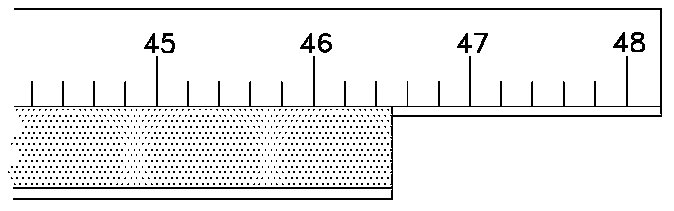
\includegraphics[width=0.5\textwidth]{./Exp1/pic/image1.png}
    \end{center}
    \caption{Measuring Length}
    \label{fig:measure}
\end{figure}

For example in the figure above, where we are measuring the length of an object against a meter stick marked in cm, we can definitely say that our result is somewhere between $46.4\,\mathrm{cm}$ and $46.6\,\mathrm{cm}$. We assume as an \emph{upper} bound of our uncertainty, an amount equal to \emph{half} this width (in this case $0.1\,\mathrm{cm}$). The final result can be written as:
\begin{equation}
    \ell = (46.5\pm 0.1)\,\mathrm{cm}
\end{equation}

\subsubsection{Estimation from the Spread (2/3 method)}

For data in which there is random uncertainty, we usually observe individual measurements to cluster around the mean and drop in frequency as the values get further from the mean (in both directions).\footnote{There is a precise mathematical procedure to obtain uncertainties (standard deviations) from a number of measured values. Here we will apply a simple ``rule of thumb'' that avoids the more complicated mathematics of that technique. The uncertainty using the standard deviation for the group of values in our example below is 0.2.}  Find the interval around the mean that contains about 2/3 of the measured points: \emph{half} the size of this interval is a good estimate of the uncertainty in each measurement. \myskip

The reasons for choosing a range that includes 2/3 of the values come from the underlying statistics of the normal (or Gaussian) distribution. This choice allows us to accurately add and multiply values with errors and has the advantage that the range is not affected much by outliers and occasional mistakes. A range that always includes all of the values is generally less meaningful. \myskip

\emph{Example}: You measure the following values of a specific quantity:
\begin{equation*}
    9.7,\:9.8,\:10,\:10.1,\:10.1,\:10.3
\end{equation*}
The mean of these six values is 10.0. The interval from 9.8 to 10.1 includes 4 of the 6 values; we therefore estimate the uncertainty to be 0.15. The result is that the best estimate of the quantity is 10.0 and the uncertainty of a single measurement is 0.2.\footnote{Note that about 5\% of the measured values will lie \emph{outside} $\pm$ twice the uncertainty}\footnote{While the above method for calculating uncertainty is good enough for our purposes, it oversimplifies a bit the task of calculating the uncertainty of the \emph{mean} of a quantity.  For those who are interested, please see the appendix for elaboration and clarification. }

\subsubsection{Square-Root Estimation in Counting}

For inherently random phenomena that involve counting individual events or occurrences, we measure only a single number $N$. This kind of measurement is relevant to counting the number of radioactive decays in a specific time interval from a sample of material, for example. It is also relevant to counting the number of left-handed people in a random sample of the population. The (absolute) uncertainty of such a single measurement, $N$, is estimated as the square root of $N$ (a counting measurement is expressed as $N \pm \sqrt{N}$). As an example, if we measure 50 radioactive decays in 1 second we should present the result as $50\pm 7$ decays per second. (The quoted uncertainty indicates that a subsequent measurement performed identically could easily result in numbers differing by 7 from 50.)

\subsection{Number of Significant Digits}

The number of significant digits in a result refers to the number of digits that are relevant. The digits may occur after a string of zeroes. For example, the measurement of $2.3\,\mathrm{mm}$ has two significant digits. This does not change if you express the result in meters as $0.0023\,\mathrm{m}$. The number 100.10, by contrast, has 5 significant digits.

When you record a result, you should use the calculated error to determine how many significant digits to keep. Let's illustrate the procedure with the following example. Assume you measure the diameter of a circle to be $d = 1.6232\,\mathrm{cm}$, with an uncertainty of $0.102\,\mathrm{cm}$. You now round your uncertainty to one or two significant digits (up to you). So (using one significant digit) we initially quote $d = (1.6232 \pm 0.1)\,\mathrm{cm}$. Now we compare the mean value with the uncertainty, and keep only those digits that the uncertainty indicates are relevant. Finally, we quote the result as $d = (1.6 \pm 0.1)\,\mathrm{cm}$ for our measurement.

Suppose further that we wish to use this measurement to calculate the circumference $c$ of the circle with the relation $c = \pi\cdot d$. If we use a standard calculator, we might get a 10 digit display indicating:
\begin{equation}
    c = 5.099433195\pm 0.3204424507\,\mathrm{cm}
\end{equation}
This is not a reasonable way to write the result!  The uncertainty in the diameter had only one significant digit, so the uncertainty of the circumference calculated from the diameter cannot be substantially better. Therefore we should record the final result as: 
\begin{equation}
    c = 5.1\pm 0.3\,\mathrm{cm}
\end{equation}
(If you do intermediate calculations, it is a good idea to keep as many figures as your calculator can store. The above argument applies when you \underline{record} your results!)

\subsection{Relative and Absolute Uncertainty}

There are two ways to record uncertainties: the absolute value of the uncertainty or the uncertainty relative to the mean value. So in the example above, you can write $c = (5.1 \pm 0.3)\,\mathrm{cm}$ or equally well $c = 5.1\,\mathrm{cm}\; (1.00 \pm 0.06)$. You can see that if you multiply out the second form you will obtain the first, since $5.1 \times 0.06 = 0.3$. The second form may look a bit odd, but it tells you immediately that the uncertainty is 6\% of the measured value. The number $0.3\,\mathrm{cm}$ is the absolute uncertainty and has the same units as the mean value (cm). The 0.06 (or 6\%) is the relative uncertainty and has no units since it is the ratio of two lengths.

\subsection{Propagation of Uncertainties}

Often, we are not directly interested in a measured value, but we want to use it in a formula to calculate another quantity. In many cases, we measure many of the quantities in the formula and each has an associated uncertainty. We deal here with how to propagate uncertainties to obtain a well-defined uncertainty on a computed quantity. 

\subsubsection{Adding/Subtracting Quantities}

When we \underline{add or subtract} quantities, their {\underline{absolute}} uncertainties must always be \underline{added} (never subtracted) to obtain the \underline{absolute uncertainty} on the computed quantity.\footnote{The propagation of random uncertainties is actually slightly more complicated, but the procedure outlined here usually represents a good approximation, and it never underestimates the uncertainty. See the appendix for more information.}

Take as an example measuring the length of a dog. We measure the distance between the left wall and the tail of the dog and subtract the distance from the wall to the dog's nose.
\begin{figure}[h]
    \begin{center}
        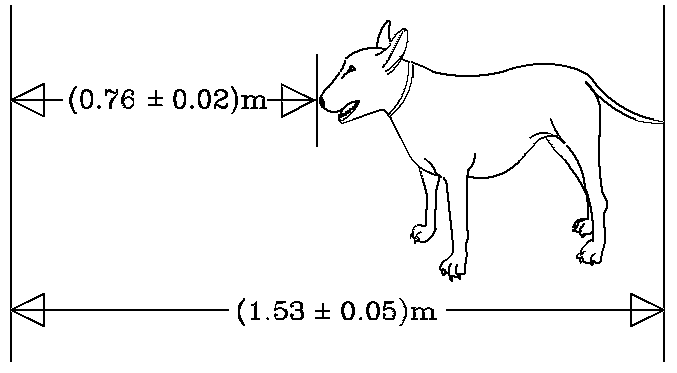
\includegraphics[width=0.5\textwidth]{./Exp1/pic/image2.png}
    \end{center}
    \caption{Measuring a Dog}
    \label{fig:dog}
\end{figure}
So the total length of the dog is:
\begin{equation}
    \begin{split}
        \text{Length} &= (1.53\pm 0.05)\,\mathrm{m} - (0.76 \pm 0.02)\,\mathrm{m} \\
        &= \left( 1.53 - 0.76 \right)\pm\left( 0.05 + 0.02 \right)\,\mathrm{m} \\
        &= \left( 0.77 \pm 0.07 \right)\,\mathrm{m}
    \end{split}
\end{equation}

\subsubsection{Multiplying/Dividing Quantities}

When we \underline{multiply or divide} quantities, we \underline{add} (never subtract) the \underline{relative uncertainties} to obtain the \underline{relative uncertainty} of the computed quantity.\footnote{Our calculation of the uncertainty actually overestimates it. The correct method does not add the absolute/relative uncertainty, but rather involves evaluating the square root of the sum of the squares. For more information please refer to the appendix of this experiment.}

Take as an example the area of a rectangle, whose individual sides are measured to be: 
\begin{align}
    a = 25.0\pm 0.5\,\mathrm{cm} = 25.0\,\mathrm{cm}\;(1.00\pm 0.02) \nonumber \\
    b = 10.0\pm 0.3\,\mathrm{cm} = 10.0\,\mathrm{cm}\;(1.00\pm 0.03)
\end{align}

The area is obtained as follows:
\begin{equation}
    \begin{split}
        \text{Area} &= \left( 25.0\pm 0.5\,\mathrm{cm} \right)\cdot\left( 10.0\pm 0.3\,\mathrm{cm} \right) \\
        &= 25.0\,\mathrm{cm}\;\left( 1.00\pm 0.02 \right)\cdot 10.0\,\mathrm{cm}\;\left( 1.00\pm 0.03 \right) \\
        &= \left( 25.0\,\mathrm{cm}\cdot 10.0\,\mathrm{cm} \right)\left( 1.00\pm \left( 0.02 + 0.03 \right) \right) \\
        &= 250.0\,\mathrm{cm}^2\;(1.00 \pm 0.05) \\
        &= 250.0\pm 12.5\,\mathrm{cm}^2 \\
        &= 250 \pm 10\,\mathrm{cm}^2
    \end{split}
\end{equation}

Note that the final step has rounded both the result and the uncertainty to an appropriate number of significant digits, given the uncertainty on the lengths of the sides. \myskip

\underline{Remarks:} Note that uncertainties on quantities used in a mathematical relationship always increase the uncertainty on the result. The quantity with the biggest uncertainty usually dominates the final result. Often one quantity will have a much bigger uncertainty than all the others. In such cases, we can simply use this main contribution. 

\subsubsection{Multiplication by a Constant}

Multiplying a value by a constant leaves the relative error unchanged. This is equivalent to multiplying the absolute error by the same constant. For example, suppose we are trying to find the circumference of a circle knowing it's radius as $r=1.0 \pm 0.1 \hspace{1mm} \text{cm}$ with error. We would calculate the circumference with error as follows.

\begin{gather}
C = 2\pi r \nonumber \\
 C= 2\pi (1.0 \pm 0.1) \\
 C=6.3 \pm 0.6 \hspace{1mm}  \text{cm} \nonumber
\end{gather}

\subsection{Numerical Statistics}
The previuos discussions of uncertainty and error tell us how we can quantitatively describe our inability to make perfect single measurements. However, in real physics experiments, very rarely do we draw conclustions from a single data points. As such, it is essential that we know how to quantify error in sets of data. The 2/3 methods as discussed in section 2.2.2 provides a good estimation of data statistics, but we can more rigorously calculate data set statistics. In statistics, a data set can be well described by the following 4 fundamental quantites: mean, median, mode, and standard deviation. The mean of a data set is the sum of all numbers in the data set divided by the number of points in the set. It is defined in the following manner.
\begin{gather}
 \text{Average} \equiv \bar x= \sum_{i} \frac{x_i}{N}
\end{gather}
The median of a data set is the middle value in a set of numbers listed in increasing order. The mode is the number that occurs the most number of times in the data set. The standard deviation decribes how the numbers in the data set are distributed around the mean. It is defined as follows.
\begin{gather}
\text{standard deviation} \equiv \sigma = \sqrt{\sum_i \frac{(x_i - \bar x)^2}{N}}
\end{gather}

These 4 statistical quantities give us enough information to characterize the distribution of our data set. For example, let's consider the two following data sets.
\myskip
\begin{center}
\begin{tabular}{c | c | c | c | c | c | c | c | c | c | c | c | c | c  }
&&&&&&&&&&Mean&Median&Mode& $\sigma$ \\
Set 1 & 9&8&11&13&10&10&12&6&9 &9.8&10&10&2.2\\
Set 2 & 11&0&10&40&2&3&10&10&4 &9.8&10&10&11.4
\end{tabular}
\end{center}
\myskip
Notice how both data sets have the same mean, median, and mode, which tells us the data points in each set are centered around the mean value of $9.8$. However, the standard deviations are quite different. The large standard deviation in data set 2 tells us there must be outliers in the data set which increase the distribution. Whereas, the relatively small standard deviation in the first data set tells us the numbers in set 1 are clustered closely togther. Standard deviation is especially important becuase it tells us exactly how distributed the number are around the mean value, which gives an indication of how error affects the spread of data points (for example, see figure \ref{fig:bellcurve} for the canonical "bell curve" distribution, also known as the gaussian distribution). The 2/3 method as discussed in section 2.2.2 is an approximation to the standard deviation since $2/3 \sim 66\%$, which roughly corresponds to the first standard deviation (see figure \ref{fig:bellcurve}).

\begin{figure}[h]
    \begin{center}
        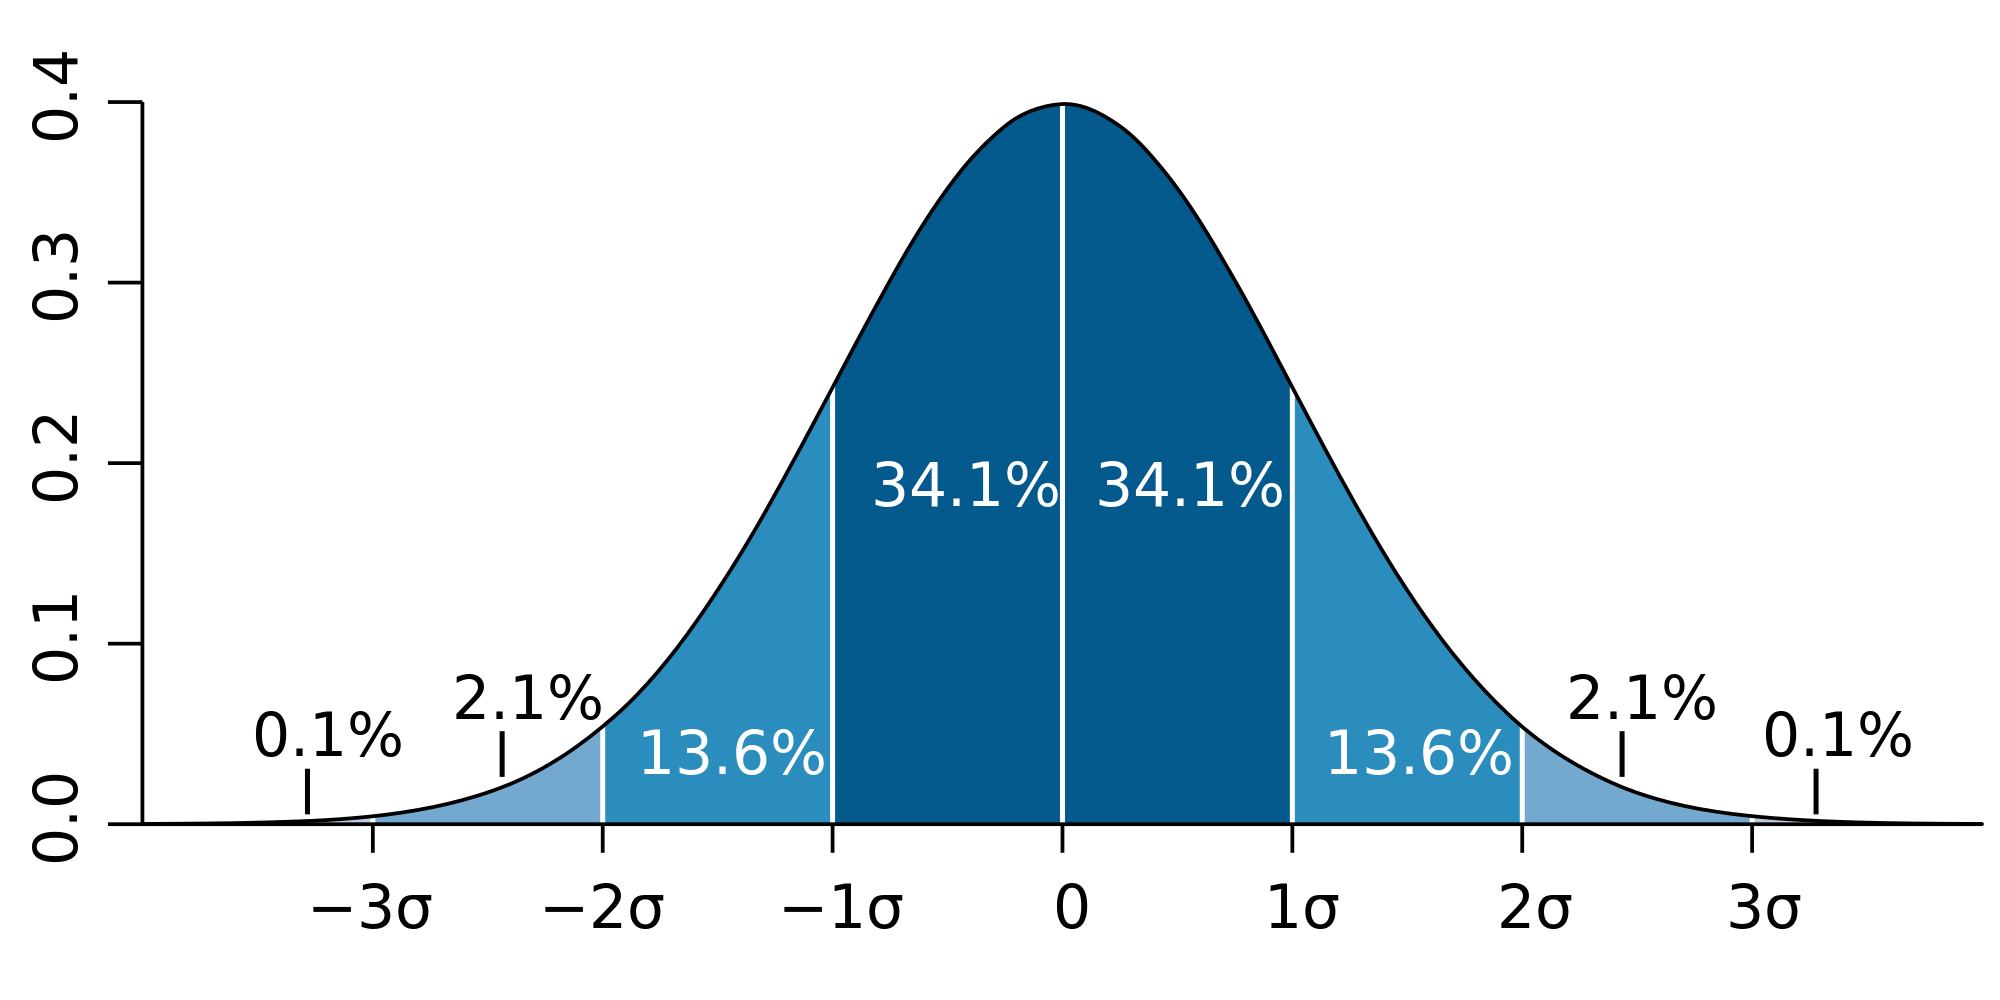
\includegraphics[width=0.7\textwidth]{./Exp0/pic/image3.png}
    \end{center}
    \caption{An example of a Gaussian distribution, also known as a bell curve. $\sim 68\%$ of the data points are within 1 standard deviation, $\sim 95\%$ of that data points are contained within 2 standard deviations, $\sim 99.5 \%$ of the data points are contained within 3 standard deviations, etc...}
    \label{fig:bellcurve}
\end{figure}

\newpage
\section{Theory-Excel}
Your TA will guide you through the relevant excel commands necessary for data analysis, however a list of some relevant excel commands are listed below. A list of all excel commands can be found on the \href{https://support.office.com/en-us/article/Excel-functions-alphabetical-b3944572-255d-4efb-bb96-c6d90033e188}{Microsoft Office website}\footnote{https://support.office.com/en-us/article/Excel-functions-alphabetical-b3944572-255d-4efb-bb96-c6d90033e188}

\begin{center}
\begin{tabular}{c | c}
ABS & Returns the absolute value of a number \\
AVERAGE & Computes the average of the selected data set \\
COS & Calculates cosine of a number\\
DEGREES & Converts radians to degrees \\
EXP & Returns e raised to the power of a given number \\
LN & Returns the natural logarithm of a number \\ 
MEDIAN & Finds the median of a data set \\
MODE.SNGL & Finds the most commonly occuring number in a data set\\
PI & Returns the value of pi\\
POWER & Returns the result of a number raised to a power\\
SIN & Calcualtes the sine of a number\\
SQRT & Calculates the square root of a number\\
STDEV.P & Calculates the standard deviation based on the entire population \\
STDEV.S & Estimates the standard deviation based on a sample \\
SUM & Calculates the sum of a data set\\
TAN & Calculates the tangent of a number
\end{tabular}
\end{center}

\section{Procedure}

\subsection{Practice with Excel Analysis}
In this section of the lab, you will get some experience using excel to determine the error on some data sets. You will need to put the data into excel and manipulate the data using the aforementioned excel commands. You can use excel on your personal computer to complete the exercises. Make sure to include the answers to the questions in your lab report.
\begin{enumerate}

\item {\bf{Data Set 1:}} consider a set of measurements you made of the gravitational constant $g$ on earth (in $m/s^2$). The data set is given below.
\begin{center}
\begin{tabular}{| c | c | c | c | c | c | c | c | c | c | c |}
\hline
Trial &1&2&3&4&5&6&7&8&9&10 \\ \hline
$g (m/s^2)$&9.7&9.2&10.1&10.0&9.5&8.9&11.1&9.8&9.7&10.0 \\
\hline
\end{tabular}
\end{center}
\begin{enumerate}
\item Calculate the mean, median, mode, and standard deviation of the data set using excel and include them in your report.
\item Estimate the error in $g$ using the 2/3 method. How does this compare to the standard deviation? 
\item Does the mean value for $g$ agree with the expected value within error? Note the standard value of $g$  is $9.81 m/s^2$.
\item If your mean doesn't agree (or if it hadn't agreed) with the expected value of $g$, what type of errors might have contributed to the incorrect value of $g$? 
\end{enumerate}

\item {\bf{Data Set 2:}} consider two sets of measurements in which you measured the length of a table that is known to be $1.25 m$. In the first method, you used a meter stick, so you had to measure twice. In the second method, you used a 2 meter stick, so you only had to measure once. Assume the ruler has centimeter precision.
\begin{center}
\begin{tabular}{ |c | c | c | c | c | c |}
\hline
Trial &1&2&3&4&5 \\ \hline
Method 1, Measurement 1 ($m$) & 1.00 & 1.00 & 1.00 &1.00 &1.00 \\
\hline
Method 1, Measurement 2  ($m$)& 0.23 &0.21&0.25&0.26&0.24 \\
\hline
Method 2 ($m$)& 1.23&1.21&1.25&1.26&1.24 \\
\hline
\end{tabular}
\end{center}
\begin{enumerate}
\item Calculate the absolute and relative uncertainties for all trials in both methods (don't use 2/3 method or standard deviation).
\item Which method is more {\it{precise}}? Which trial is more {\it{accurate}}?
\item Estimate the error using the 2/3 methods. How does this compare to the error you calculated in part (a).
\item What could you conclude about making measurements with a ruler?
\end{enumerate}

\item {\bf{Data Set 3:}} consider a measurement you made in which you counted the number of cars that passed in 1 hour on various highways in the united states. The data set containing the number of cars per hour is given in the following table.
\begin{center}
\begin{tabular}{|c | c | c | c | c | c | c | c | c | c | c|}
\hline
Trail&1&2&3&4&5&6&7&8&9&10 \\ \hline
$N_{\text{cars}}$&523&143&496&1045&869&57&693&1150&327&87 \\
\hline
\end{tabular}
\end{center}
\begin{enumerate}
\item Calculate the absolute error and the relative error in each measurement.
\item Which trial has the lowest absolute error?
\item Which trial has the lowest relative error?
\item Which trial would you say is the most precise?
\item Calculate the rate in cars {\it{per second}} for each measurement with error.
\item What experimental factors might contribute to the error in car rate (be creative!)?
\end{enumerate} 
\end{enumerate}


\section{Applications}
You read of a certain test intended to indicate a particular kind of cancer. The test gives you a positive result for $(80 \pm 10) \%$ of all persons tested who really have this kind of cancer (true positives). But the test also gives you a positive result for $(2 \pm 1) \%$ of all healthy persons (false positives). Now you read a publication where the author performed this test on $10,000$ workers that deal with a certain chemical. The author got 400 positive samples from these workers and claims that this is strong evidence that this particular chemical enhances the development of this kind of cancer since it is known from literature that only $(1 \pm 0.5)\%$ of the population are expected to have this kind of cancer. How reliable is the claim of the author?\myskip

\noindent \underline{Numerical Answer}:

If one assumes that the 10,000 workers would mirror the average population, then there should be:
\begin{equation}
    10000 \times (0.010 \pm 0.005) = 100 \pm 50
\end{equation}
persons having this cancer. Of them, the test gives:
\begin{equation}
    (0.8 \pm 0.1) \times (100 \pm 50) = 80 \pm 50
\end{equation}
positive results (true positives).\myskip

There are then $9900 \pm 50$ persons expected not to have this kind of cancer. Of them:
\begin{equation}
    (0.02 \pm 0.01) \times (9900 \pm 50) \approx 200 \pm 100
\end{equation}
give positive results (false positives).\myskip

The total number of positives in the average population is therefore $280 \pm 150$.\myskip

So how do you judge the author's conclusion of ``strong evidences''?\myskip

If you wanted to design a new test using the same procedure but to arrive at a stronger conclusion, and you could either increase the rate of true positives or decrease the rate of wrong negatives, which would you choose?\myskip

\noindent\emph{Reference}: Paul Cutler: Problem Solving in Clinical Medicine, Chapter 5, Problem 5 (modified).


